\chapter{Chapter 5. Semantics for Propositional Logic}

\section*{5.5 Self-Study Questions}



	\begin{enumerate}
	
		\item[5.5.1] We can't predict the number of rows because we don't know how many sentence letters are there in the formula.  (Well, to be super precise, there will be at least one row and at most $2^4=16$ rows. The former in case there is only one letter the latter in case there are 4, which is the most you can have with 3 connectives)
		
		
		\item[5.5.2] (a) would mean that $\phi\land\psi=p\land\neg p$ and we've checked that $p\land\neg p$ is a contradiction. (b) is the only sensible option and it's easily checked that if $\vDash \phi$ and $\vDash\psi$, then $\vDash\phi\land \psi$. (c) would mean that $\phi\land\psi$ is also of the form $\phi\lor\psi$, which is impossible. (d) doesn't make sense. 
	
		\item[5.5.3] (a) entails that $\vDash\phi\to\psi$ by the deduction theorem. (b) entails that $\vDash\phi\to\psi$ by the observation that if $\llbracket\psi\rrbracket_v=1$ for all valuations, then also $\llbracket \phi\to\psi\rrbracket_v=max(1-\llbracket\phi\rrbracket_v,\llbracket\psi\rrbracket_v)=1$ for all valuations $v$ . (c) follows from the fact that $\neg\psi\to\neg\phi\equi\phi\to\psi$ by the law of contraposition. And (d) follows from the observation that that if $\llbracket\neg \phi\rrbracket_v=1$ for all valuations, then $\llbracket \phi\rrbracket_v=0$ and so $\llbracket \phi\to\psi\rrbracket_v=max(1-\llbracket\phi\rrbracket_v,\llbracket\psi\rrbracket_v)=1$ for all valuations $v$.
	
	\end{enumerate}

\section*{5.6 Exercises}

	\begin{enumerate}

      \item[5.6.2]

        \begin{enumerate}[(i)]
            \setcounter{enumii}{14}
          \item We want to show that for all $\phi, \psi,$ and $\theta$, we have
            \[\phi \vee (\psi \wedge \theta) \equi (\phi \vee \psi) \wedge (\phi \vee \theta)\]

            We'll prove this directly.
            We know that
            $\phi \equi \psi$
            iff for all valuations $v$,
            $\llbracket \phi \rrbracket_v = \llbracket\psi\rrbracket_v$
            (see proposition 5.2.5).

            Let's apply the truth functions to our formulas with an arbitrary valuation $v$:
           \begin{align*}
\llbracket \phi\vee (\psi\wedge\theta)\rrbracket_v &= max(\llbracket\phi\rrbracket_v \, , \, \llbracket \psi \wedge \theta \rrbracket_v ) \\
& = max(\llbracket\phi\rrbracket_v \, , \, min(\llbracket \psi \rrbracket_v, \llbracket \theta \rrbracket_v ))\\\\
\llbracket (\phi\vee\psi) \wedge (\phi \vee \theta)\rrbracket_v &= min(\llbracket\phi\vee\psi\rrbracket_v \, , \, \llbracket \phi \vee \theta \rrbracket_v ) \\
& = min(max(\llbracket\phi\rrbracket_v \, , \, \llbracket\psi\rrbracket_v) \, , \, max(\llbracket \phi \rrbracket_v\, , \, \llbracket \theta \rrbracket_v ))
           \end{align*}


            We have to prove that for all $x,y,z\in \{0,1\}$, we have:
            \[max(x, min(y,z)) = min(max(x,y),max(x,z))\]

            We distinguish two cases:
            (i) $x = 0$ and
            (ii) $x = 1$.
            \begin{itemize}
              \item[(i)] Assume $x=0$.
                Then we have
                $max(x,y) = y$
                and
                $max(x,z) = z$.
                Substituting this in the identity
                $min(max(x,y),max(x,z)) =min(max(x,y),max(x,z))$
                gives us
                $min(max(x,y) \, , \, max(x,z)) = min (y,z)$.
                And if $x=0$ we also know that
                $max(x \, , min(y,z)) = min(y,z)$.
                It follows that
                $max(x, min(y,z)) = min(max(x,y), max(x,z))$.
                So, in case (i) the claimed equation holds.

              \item[(ii)]  Assume that $x=1$.
                It follows that
                $max(x, min(y,z)) = x=1$.
                We also get that
                $max(x,y) = max(x,z) = x=1$.
                So,
                $min(max(x,y), max(x,z)) = 1$.
                It follows immediately that
                $max(x, min(y,z)) = min(max(x,y), max(x,z))$,
                which is what we wanted to show.
            \end{itemize}
            So, what we've shown is that for all values $x,y,z\in\{0,1\}$, our equation holds.
            This gives us quickly that for all \emph{valuations}
            $v:\mathcal{P}\to\{0,1\}$,
            we have that
            $\llbracket \phi \vee (\psi \wedge \theta) \rrbracket_v = \llbracket(\phi \vee \psi) \wedge (\phi \vee \theta)\rrbracket_v$,
            which entails our claim.

        \end{enumerate}

		\item[5.6.3] 

		\begin{enumerate}[(i)]
		
			\setcounter{enumii}{2}
			
			\item \emph{Claim}. For all $\Gamma,\Delta\subseteq\mathcal{L}$ and $\phi\in\mathcal{L}$, we have if $\Gamma\vDash\phi$, then $\Gamma\cup\Delta\vDash\phi$.
			
			\begin{proof}
			We prove this by conditional proof. So let $\Gamma,\Delta\subseteq\mathcal{L}$ and $\phi\in\mathcal{L}$ be arbitrary and assume that $\Gamma\vDash\phi$. This means that for all valuations $v$, if $v$ makes all the members of $\Gamma$ true, then $v$ makes $\phi$ true. We want to show that $\Gamma\cup\Delta\vDash\phi$, i.e. if a valuation $v$ makes all the members of  $\Gamma\cup\Delta$ true, then $v$ makes all the members of $\phi$ true. So let $v$ be an arbitrary valuation that makes all the members of  $\Gamma\cup\Delta$ true. Since $\Gamma\subseteq\Gamma\cup\Delta$, it follows that $v$ makes all the members of $\Gamma$ true. But by assumption ($\Gamma\vDash\phi$), this means that $v$ makes $\phi$ true, which is what we needed to show.
			\end{proof}
		
			\setcounter{enumii}{12}
			
			\item \emph{Claim}. $(\phi\lor\psi)\lor\theta\equi \phi\lor(\psi\lor\theta)$
			
			\begin{proof}
			There are different ways of proving this. The easiest is via Proposition 5.2.5. Remember that this Proposition states that $\phi\equi\psi$ iff for all valuations $v$, $\llbracket\phi\rrbracket_v=\llbracket\psi\rrbracket_v$. Now consider $\llbracket(\phi\lor\psi)\lor\theta\rrbracket_v$ and $\llbracket\phi\lor(\psi\lor\theta)\rrbracket_v$ for an arbitrary valuation $v$. We have $\llbracket(\phi\lor\psi)\lor\theta\rrbracket_v=max(\llbracket(\phi\lor\psi)\rrbracket_v, \llbracket\theta\rrbracket_v)=max(max(\llbracket\phi\rrbracket_v,\llbracket\psi\rrbracket_v), \llbracket\theta\rrbracket_v)$ and $\llbracket \phi\lor(\psi\lor\theta)\rrbracket_v=max(\llbracket\phi\rrbracket_v, \llbracket\psi\lor\theta\rrbracket_v)=max(\llbracket\phi\rrbracket_v,max(\llbracket\psi\rrbracket_v, \llbracket\theta\rrbracket_v))$. The claim follows immediately from the (combinatoric) observation that for all $x,y,z\in\{0,1\}$, $max(max(x,y),z)=max(x,max(y,z))$. This observation can be proven in many ways, here's one. We distinguish two cases: (a) $x=y=z=0$ and (b) at least one of $x,y,z$ is 1. In case (a), \[max(max(x,y),z)=max(max(0,0),0)=max(0,0)=0\]\[max(x,max(y,z))=max(0,max(0,0))=max(0,0)=0\] If at least one of $x,y,z$ is 1, then either $max(x,y)=1$ or $z=1$, hence $max(max(x,y),z)=1$. Similarly, if at least one of $x,y,z$ is 1, then either $x=1$ or $max(y,z)=1$, so $max(x,max(y,z))=1$. Hence, either way, $max(max(x,y),z)=max(x,max(y,z))$, as desired.
			\end{proof}
			
			
			\setcounter{enumii}{14}
			
			\item \emph{Claim}. $\phi\lor(\psi\land\theta)\equi (\phi\lor\psi)\land(\phi\lor\theta)$
			
			\begin{proof}
			 
			 Again, there are several ways of doing this. We show this directly, i.e. we show that (1) $\phi\lor(\psi\land\theta)\vDash (\phi\lor\psi)\land(\phi\lor\theta)$ and (2) $(\phi\lor\psi)\land(\phi\lor\theta)\vDash\phi\lor(\psi\land\theta)$ from definitions. We proceed in turn:
			 
			 \begin{enumerate}[1.]
			 
			 	\item We want to show that $\phi\lor(\psi\land\theta)\vDash (\phi\lor\psi)\land(\phi\lor\theta)$, i.e. if $\phi\lor(\psi\land\theta)$ is true under a valuation $v$, then  $(\phi\lor\psi)\land(\phi\lor\theta)$ is also true under $v$. So, suppose that $\llbracket \phi\lor(\psi\land\theta)\rrbracket_v=1,$ for an arbitrary valuation $v$. We know that $\llbracket \phi\lor(\psi\land\theta)\rrbracket_v=max(\llbracket\phi\rrbracket_v, \llbracket (\psi\land\theta)\rrbracket_v)=max(\llbracket\phi\rrbracket_v, min(\llbracket \psi\rrbracket_v,\llbracket\theta\rrbracket_v)$. Since $\llbracket \phi\lor(\psi\land\theta)\rrbracket_v=1$, we can distinguish two cases: (a) $\llbracket\phi\rrbracket_v=1$ or (b) $min(\llbracket \psi\rrbracket_v,\llbracket\theta\rrbracket_v)=1$. In case (a), we can infer that $\llbracket \phi\lor\psi)\rrbracket_v=max(\llbracket\phi\rrbracket_v,\llbracket\psi\rrbracket_v)=1$ and $\llbracket \phi\lor\theta)\rrbracket_v=max(\llbracket\phi\rrbracket_v,\llbracket\theta\rrbracket_v)=1$. Hence $\llbracket (\phi\lor\psi)\land(\phi\lor\theta)\rrbracket_v=min(\llbracket \phi\lor\psi)\rrbracket_v, \llbracket \phi\lor\theta)\rrbracket_v)=1,$ as desired. In case (b), we can infer that both $\llbracket \psi\rrbracket_v=1$ or $\llbracket\theta\rrbracket_v)=1$. Hence both $\llbracket \phi\lor\psi)\rrbracket_v=max(\llbracket\phi\rrbracket_v,\llbracket\psi\rrbracket_v)=1$ and $\llbracket \phi\lor\theta\rrbracket_v=max(\llbracket\phi\rrbracket_v,\llbracket\theta\rrbracket_v)=1$; so we get $\llbracket (\phi\lor\psi)\land(\phi\lor\theta)\rrbracket_v=min(\llbracket \phi\lor\psi)\rrbracket_v, \llbracket \phi\lor\theta)\rrbracket_v)=1,$ again as desired. So, in either case, $\llbracket (\phi\lor\psi)\land(\phi\lor\theta)\rrbracket_v=1$ proving our claim that $\phi\lor(\psi\land\theta)\vDash (\phi\lor\psi)\land(\phi\lor\theta)$.
				
				\item We want to show that $(\phi\lor\psi)\land(\phi\lor\theta)\vDash\phi\lor(\psi\land\theta)$. So, suppose that $\llbracket (\phi\lor\psi)\land(\phi\lor\theta)\rrbracket_v=1$ for some arbitrary valuation $v$. Since $\llbracket (\phi\lor\psi)\land(\phi\lor\theta)\rrbracket_v=min(\llbracket \phi\lor\psi)\rrbracket_v, \llbracket \phi\lor\theta)\rrbracket_v)$, it follows that both $\llbracket \phi\lor\psi\rrbracket_v=1$ and $\llbracket \phi\lor\theta\rrbracket_v=1$. We can easily see that there are two cases to consider, (a) $\llbracket\phi\rrbracket_v=1$ and (b) both 
			 $\llbracket\psi\rrbracket_v=1$ and $\llbracket\theta\rrbracket_v=1$. In case (a), we easily get $\llbracket \phi\lor(\psi\land\theta)\rrbracket_v=max(\llbracket\phi\rrbracket_v, \llbracket (\psi\land\theta)\rrbracket_v)=1$. In case (b), we first note that we get  $\llbracket\psi\land\theta\rrbracket_v=min(\llbracket \psi\rrbracket_v,\llbracket\theta\rrbracket_v)=1$. From this, by $\llbracket \phi\lor(\psi\land\theta)\rrbracket_v=max(\llbracket\phi\rrbracket_v, \llbracket (\psi\land\theta)\rrbracket_v)$, it quickly follows that $\llbracket \phi\lor(\psi\land\theta)\rrbracket_v=1$. So, either way, $\llbracket \phi\lor(\psi\land\theta)\rrbracket_v=1$, which is what we needed to show.
			 \end{enumerate}
			
			\end{proof}
			
					\end{enumerate}

			
%		\item[5.6.4] We prove this by induction on formulas. 
%		
%			\begin{enumerate}[(i)]
%			
%				\item \emph{Base case}. A sentence letter clearly doesn't contain any $\neg$'s, so the case is trivially satisfied. 
%				
%				\item \emph{Induction steps}:
%				
%				\begin{enumerate}[(a)]
%				
%					\item Assume the induction hypothesis that $\phi$ does not contain any $\neg$'s. Consider $\neg\phi$. Since 
%									
%				\end{enumerate}
%			
%			\end{enumerate}
			
		\item[5.6.5] We prove this claim by contradiction. Suppose that there is a valuation $v$, such that $\llbracket\phi\rrbracket_v=1$ for all $\phi\in\mathcal{L}$. It follows that $\llbracket p\rrbracket_v=1$ and $\llbracket\neg p\rrbracket_v=1$ (since both $p,\neg p\in\mathcal{L}$). But  then, also $\llbracket\neg p\rrbracket_v=1-\llbracket p\rrbracket_v=0$. Contradiction! Hence there is no valuation $v$, such that $\llbracket\phi\rrbracket_v=1$ for all $\phi\in\mathcal{L}$.
		

		\item[5.6.7]
		
		\begin{enumerate}[(a)]
		
			\item $p \lor (q \land r) \leftrightarrow (p \lor q) \land(p \lor r)$
			
			\begin{center}
			\emph{Parsing Tree}:\\[1ex]
			
				\begin{tikzpicture}
				\Tree [.{$p \lor (q \land r) \leftrightarrow (p \lor q) \land(p \lor r)$} [.{$p \lor (q \land r)$} [.$p$ ] [.{$q\land r$} [.$q$ ] [.$r$ ] ] ] [.{$(p \lor q) \land(p \lor r)$} [.{$p \lor q$} [.$p$ ] [.$q$ ] ] [.{$p \lor r$} [.$p$ ] [.$r$ ] ]  ]  ]
				\end{tikzpicture}\\[2ex]
				
			\emph{Truth Table}:\\[2ex]
			
			{\tiny\begin{tabular}{c c c | c | c  c  c  c  c}
$p$ & $q$  & r & $q\land r$ & $p \lor (q \land r)$ & $p\lor q$ & $p\lor r$ & $(p \lor q) \land(p \lor r)$ & $p \lor (q \land r) \leftrightarrow (p \lor q) \land(p \lor r)$ \\\hline

1 & 1 & 1 & 1 & 1&1&1&1& 1\\

1 & 1 & 0 & 0& 1&1&1&1&  1\\

1 & 0 & 1 & 0 & 1&1&1&1& 1\\

1 & 0 & 0  & 0 &1 &1&1& 1& 1\\

0 & 1 &  1 & 1 &1 &1&1& 1& 1\\

0 & 1 & 0 & 0&0 & 1&0&0& 1 \\

0 & 0 & 1 & 0 & 0& 0&1&0& 1  \\

0 & 0 & 0 & 0 & 0& 0&0&0& 1

\end{tabular}}

\vspace{2ex}

\end{center}

		\setcounter{enumii}{6}
		
		\item 
		
		\Tree [.${(\neg p \lor q) \rightarrow (q \land (p \leftrightarrow q))}$ [.${(\neg p \lor q)}$ [.$\neg p$ [.$p$ ] ] [.$q$ ] ] [.${q \land (p \leftrightarrow q)}$ [.$q$ ] [.$p\leftrightarrow q$ [.$p$ ] [.$q$ ] ] ] ]

\begin{tabular}{cc|c|c|c|c|c||c|}

$p$&$q$& $p\leftrightarrow q$ &  $\neg p$ & $\neg p \lor q$ & $q\land (p\leftrightarrow q)$  & $(\neg p \lor q) \rightarrow (q \land (p \leftrightarrow q))$\\\hline

	1 & 1 &1 & 0 & 1&1&1\\\hline
	
	1 & 0 & 0 & 0& 0& 0&1\\\hline
	
	0 & 1 & 0 & 1& 1& 0& 0\\\hline
	
	0 & 0 & 1 & 1& 1& 0& 0 \\


\end{tabular}
		
			\setcounter{enumii}{16}
		
		\item 
		
		\Tree [.${p \to (q \to (r \to (\neg p \to (\neg q \to \neg r))))}$ [.$p$ ] [.${(q \to (r \to (\neg p \to (\neg q \to \neg r))))}$ [.$q$ ] [.${(r \to (\neg p \to (\neg q \to \neg r)))}$ [.$r$ ] [.$\neg p\to(\neg q\to\neg r)$ [.$\neg p$ [.$p$ ] ] [.$\neg q\to\neg r$ [.$\neg q$ [.$q$ ] ] [.$\neg r$ [.$r$ ] ] ] ] ] ] ] 
		
		Truth table on next page:

\newpage

		
		\end{enumerate}
		
	
		
	
	\end{enumerate}


\begin{landscape}
\begin{center}
\small
\begin{tabular}{ccc|c|c|c|c|c|c|c|c|}
$p$&$q$&$r$& $\neg q$ & $\neg r$ & $\neg q\to\neg r$ & $\neg p$ & $\neg p\to (\neg q\to \neg r)$ & $r\to(\neg p\to (\neg q\to \neg r))$ & $q\to(r\to(\neg p\to (\neg q\to \neg r)))$ & $p \to (q \to (r \to (\neg p \to (\neg q \to \neg r))))$ \\
\hline
 1 & 1 & 1 &0 &0 &1 &0 &1 &1 &1 &1 \\\hline
 1 & 1 & 0 &0 &1 &1 &0 &1 &1 &1 &1 \\\hline
 1 & 0 & 1 &1 &0 &0 &0 &1 &1 &1 &1 \\\hline
 1 & 0 & 0 &1 &1 &1 &0 &1 &1 &1 &1 \\\hline
 0 & 1 & 1 &0 &0 &1 &1 &1 &1 &1 &1 \\\hline
 0 & 1 & 0 &0 &1 &1 &1 &1 &1 &1 &1 \\\hline
 0 & 0 & 1 &1 &0 &0 &1 &0 &0 &1 &1 \\\hline
 0 & 0 & 0 &1 & 1&1 &1 &1 &1 &1 &1 \\
\end{tabular}
\end{center}
\end{landscape}

\newpage

\begin{enumerate}

	\item[] \begin{enumerate}[(a)]
	
	\setcounter{enumii}{18}
	
		\item 
		
		\Tree [.${p \land (\neg p \lor q) \to (r \to \neg q) \land (p \to r)}$ [.${p \land (\neg p \lor q)}$ [.$p$ ] [.$\neg p\lor q$ [.$\neg p$ [.$p$ ] ] [.$q$ ] ] ] [.${(r \to \neg q) \land (p \to r)}$ [.$r\to\neg q$ [.$r$ ] [.$\neg q$ [.$q$ ] ] ] [.$p\to r$ [.$p$ ] [.$r$ ] ] ] ]
		
			
	Truth-table on next page.		
	\end{enumerate}
	
	

	

\end{enumerate}

\begin{landscape}
\begin{tabular}{ccc|c|c|c|c|c|c|c|c|}

$p$&$q$&$r$& $\neg p$ & $\neg q$ & $\neg p\lor q$ & $r\to\neg q$ & $p\to r$ & $p\land (\neg p\lor q)$ & ${(r \to \neg q) \land (p \to r)}$ & ${p \land (\neg p \lor q) \to (r \to \neg q) \land (p \to r)}$ \\
\hline
 1 & 1 & 1 & 0 &  0 &1 &0 &1 &1 &0 &0 \\\hline
 1 & 1 & 0 & 0 & 0 &1 &1 &0 &1 &0 &0 \\\hline
 1 & 0 & 1 & 0 & 1 &0 &1 &1 &0 &1 &1\\\hline
 1 & 0 & 0 & 0 & 1 &0 &1 &0 &0 &0 &1\\\hline
 0 & 1 & 1 &  1 &0 &1 &0 &1 &0 &0 &1\\\hline
 0 & 1 & 0 & 1 & 0 &1 &1 &1 &0 &1 &1\\\hline
 0 & 0 & 1 & 1 & 1 &1 &1 &1 &0 &1 &1\\\hline
 0 & 0 & 0 & 1 & 1 &1 &1 &1 &0 &1 &1\\\hline
\end{tabular}
\end{landscape}
			
\begin{enumerate}		

		\item[5.6.8]
		
		\begin{enumerate}[(a)]
		
			\item We know that $p\therefore p\lor (p\land q)$ is valid iff $p\vDash p\lor (p\land q)$. By the deduction theorem, the latter is equivalent to $\vDash p\to( p\lor (p\land q))$. This we can check via truth-tables. Here we go:
			
			\begin{center}
			\emph{Parsing Tree}:\\[1ex]
			
				\begin{tikzpicture}
				\Tree [.{$p\to( p\lor (p\land q))$} [.$p$ ] [.{$p\lor (p\land q)$} [.$p$ ] [.$p\land q$ [.$p$ ] [.$q$ ] ] ] ]
				\end{tikzpicture}\\[2ex]
				
			\emph{Truth Table}:\\[1ex]
			
			\begin{tabular}{c c | c c c}
			 $p$ & $q$ & $p\land q$ & $p\lor (p\land q)$ & $p\to (p\lor (p\land q)$\\\hline
			 
			 1 & 1 & 1 & 1& 1\\
			 1 & 0& 0& 1& 1 \\
			 0 & 1& 0& 0& 1\\
			 0& 0 & 0& 0& 1\\
			 
			
			\end{tabular}
			
			\end{center}
		
		Since there are only $1$'s in the final column, the formula is a logical truth and the argument therefore valid.


	\end{enumerate}
	
	

	

\end{enumerate}
	
%%% Local Variables: 
%%% mode: latex
%%% TeX-master: "../../logic.tex"
%%% End:
